\documentclass[12pt,a4paper]{article}
\usepackage[UTF8]{ctex} % 支持中文
\usepackage{geometry}
\usepackage{graphicx}
\usepackage{amsmath}
\usepackage{float}
\usepackage{subfigure}
\usepackage{booktabs} % 表格美化
\usepackage{cite}
\usepackage{ulem}
\usepackage{array}
\usepackage{multirow}
\usepackage{hanging}


\newcolumntype{M}[1]{>{\centering\arraybackslash}m{#1}}
\newcommand{\down}[2]
{
	$\Delta_{\text{#1}}\approx{#2}$
}

% 设置页面边距
\geometry{left=2.5cm,right=2.5cm,top=2.5cm,bottom=2.5cm}

\title{\Huge{\textbf{\uuline{实\ 验\ 报\ 告}}}}
\author{\uline{少年班}\ 学院 \quad 姓名:\ \uline{顾泓宇} \quad 学号:\ \uline{PB23000078} \quad 实验日期:\ \uline{2024-9-20} }
\date{}

\begin{document}
	\maketitle

	\section{实验题目}
	测量金属丝的杨氏模量和泊松比
	
	\section{基本原理}
	\subsection{金属丝的杨氏模量和泊松比}
	杨氏模量是材料的重要力学参数，反映了材料抵抗形变能力的大小。拉力F
	与丝的原始横截面A之比定义为应力，伸长量L与丝的原始长度 $\Delta L$ 之比定义为纵向线应变。在弹性范围内，应力与应变满足胡克定律：\\
	\begin{center}
		$\frac{F}{A}=E \frac{\Delta L}{L}$
	\end{center}
	其中 E 为材料的杨氏模量，用砝码拉伸金属丝提供F.\\
	式（1）中只考虑了材料的微小纵向应变，忽略了横向变化。横向变化量$\Delta d$
	与丝的原始横向长度 d 之比定义为横向线应变。在实践中，纵向拉伸应变还会导致横向收缩应变。实验表明，在材料弹性范围内，横向线应变$\frac{\delta d}{d}$与纵向线应变之比$\frac{\Delta L}{L}$为常数：\\
	\begin{center}
		$\frac{\Delta d}{d}=-\mu \frac{\Delta L}{L}$
	\end{center}
	(2)式中的负号表示纵向拉伸导致横向收缩，$\mu$为横向变形系数或称泊松比。\\
	式（2）中的$\Delta d$太小，因此本实验无法直接测量$\mu$，但可通过非平衡电桥测量金属丝经拉伸后的微小电阻变化而间接得到。
	\subsection{非平衡电桥}
	非平衡电桥与传感器配合使用，可测量温度、应力、位移等物理量。图 1 为非平衡电桥的原理图，其中电阻箱 $R_1$、$R_2$、$R_3$为电桥的三个臂，电阻箱 $R_4$与待测金属丝电阻 $R_s$ 串联构成第四臂，$R_0$ 为电位器，C 是滑动头。\\
	\begin{center}
		
\includegraphics[width=0.6\textwidth]{figs/3.png}\\
		图一：非平衡电桥
	\end{center}
	当电桥平衡时：\\
	\begin{center}
		$\frac{R_1}{R_2}=\frac{R_3}{R_4+R_s}$
	\end{center}
	任意桥臂阻值变化时，电桥将偏离平衡位置。金属丝受到拉伸引起电阻变化$\Delta R_s$,当$R_4+R_s$的相对阻值变化量小于$1\%$时，桥电压$U_g$(即D,E之间的电压)与该桥臂的电阻变化量近似满足线性关系：\\
	\begin{center}
		$U_g\approx \frac{U_AC}{4}\cdot \frac{\Delta R_s}{R_4+R_s}$
	\end{center}
	即将电阻的微小变化量转化成直流电压信号进行测量。\\
	本实验的研究对象为金属丝。
	
	\section{基础内容}
	实验中路端电压为0.5V,L=117.5cm,$R_s\approx 7.285\Omega$
	\begin{center}
		\begin{tabular}{|M{6em}|M{6em}|M{6em}|}\hline
			砝码质量m/g & 桥电压$U_g$/mV & 伸长量$\Delta L$/mm    \\\hline
			99.63 & 0.097 & 0.190   \\\hline
			199.71 & 0.128 & 0.315   \\\hline
			299.52 & 0.161 & 0.450   \\\hline
			399.79 & 0.197 & 0.550   \\\hline
			499.53 & 0.216 & 0.678   \\\hline
			599.48 & 0.227 & 0.853   \\\hline
			699.42 & 0.243 & 0.961   \\\hline
			799.43 & 0.302 & 1.075   \\\hline
			899.44 & 0.441 & 1.223   \\\hline
			999.61 & 0.496 & 1.360   \\\hline
		\end{tabular}
	\end{center}
	\begin{center}
		表一：砝码质量，桥电压与伸长量测量数据
	\end{center}
	\subsection{金属丝杨氏模量}
	利用最小二乘法对m与$\Delta L$进行线性拟合，结果如下：\\
	\begin{center}
		
\includegraphics[width=1\textwidth]{figs/1.png}\\
		图二：砝码质量m与伸长量$\Delta L$线性拟合
	\end{center}
	\large
	则$\frac{EA}{gL}=770$,算得金属丝杨氏模量E=$\frac{770\cdot 9.795\cdot 1.175}{\pi d^2/4}=125.43GPa$\\
	\subsection{金属丝泊松比}
	由
	\begin{center}
		$R_s=\rho \frac{L}{A}$\\
		$\frac{\Delta d}{d}=-\mu \frac{\Delta L}{L}$
	\end{center}
	则$U_g=\frac{(1+2\mu)R_sU_{AC}}{4(R_4+R_s)\cdot L}\cdot \Delta L$\\
	利用最小二乘法对$U_g$与$\Delta L$进行线性拟合，结果如下：\\
	\begin{center}
		
\includegraphics[width=1\textwidth]{figs/2.png}\\
		图三：砝码质量m与伸长量$\Delta L$线性拟合
	\end{center}
	\large
	则$U_g=0.31\Delta L+0.01$,算得金属丝泊松比$\mu=0.4$
	
	\subsection{温差电效应}
	对高电势一端焊点哈气，$U_g$增加，对低电势一端哈气，$U_g$降低\\
	原因：哈气引起的两端温度变化，在金属丝两端引起温差电动势。
	
	\section{附录}
	原始数据如下图四：\\
	\begin{center}
		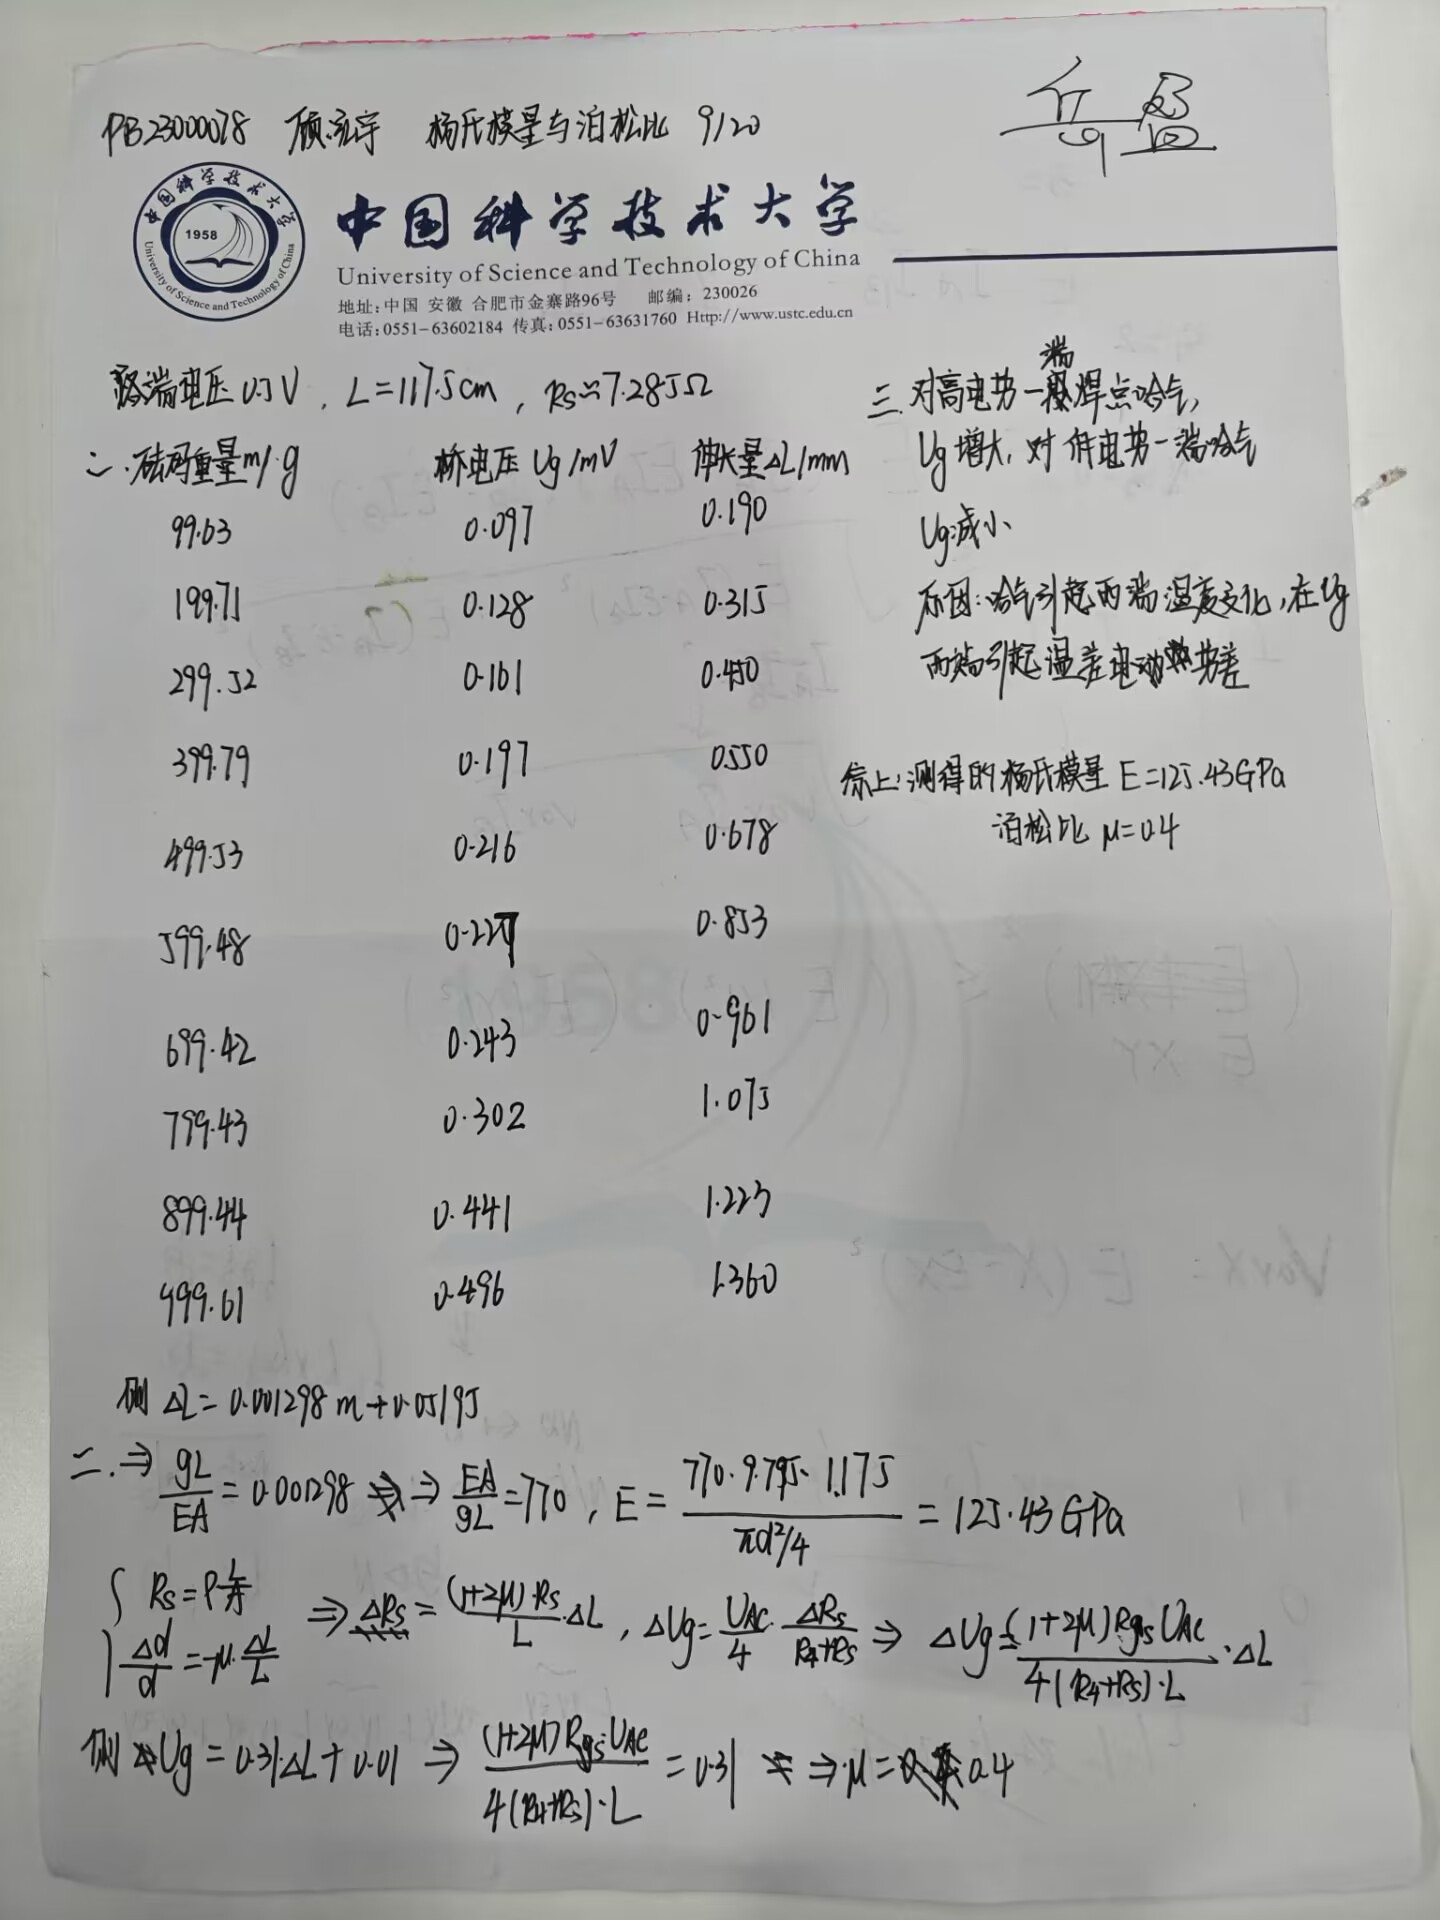
\includegraphics[width=0.7\textwidth]{figs/4.jpg}\\
		图四：原始数据记录
	\end{center}
	
	\section{参考文献}
	[1]. 测量金属丝的杨氏模量和泊松比. 实验讲义.2024
\end{document}